\newpage
\section{Realizacja prototypu}
\label{sec:realizacja}

\subsection{Architektura prototypu}
\label{subsec:architektura_prototypu}

Zaimplementowany finalny system asystenta głosowego Wilga odpowiada oparty jest na koncepcji
z~rozdziału~\ref{subsec:przeplyw}, składają się na nią: aplikacja użytkownika, serwer orkiestrujący
oraz węzeł brzegowy Raspberry~Pi~5. Schemat wdrożenia przedstawiono
na rysunku~\ref{fig:architektura}, zastosowano ten sam podział na trzy
środowiska co na rysunku schematu testowego~\ref{fig:schemat}, w przypadku prezentowanej wdrożeniowej wersji asystenta przedstawiono architekturą wraz z~konkretnymi procesami i~kierunkami przepływu danych.

\begin{figure}[H]
    \centering
    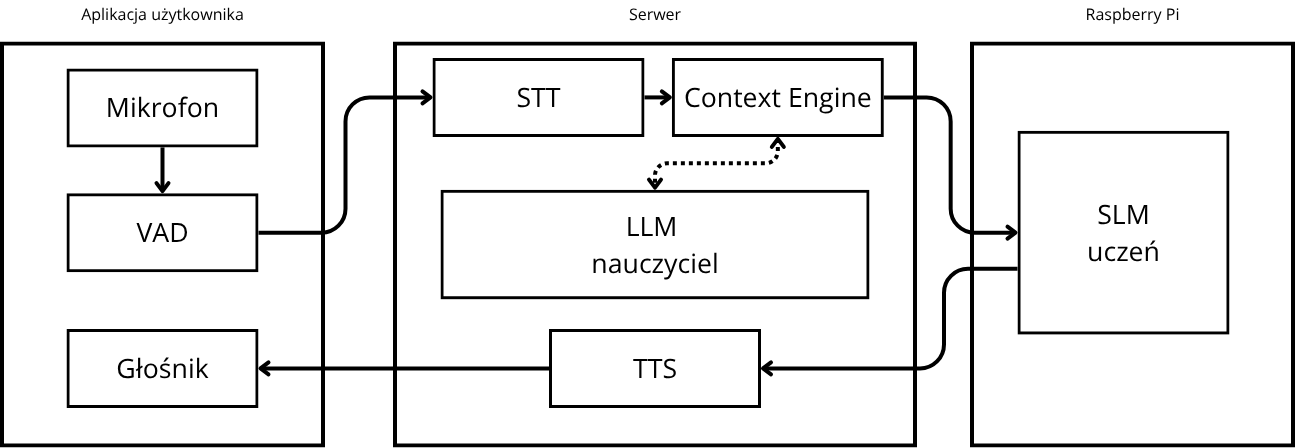
\includegraphics[width=\textwidth]{src/img/system-schemat.png}
    \caption{Architektura prototypu Wilga --- przepływ danych od mikrofonu
             do głośnika. Linia przerywana oznacza asynchroniczną współpracę
             Context Engine z~modelem Nauczyciela.}
    \label{fig:architektura}
\end{figure}

Architektura produkcyjna jest pokrewna, lecz nie tożsama z~układem
benchmarkowym opisamym w sekcji~\ref{subsec:metodologia} (rysunek~\ref{fig:testy_arch}).
Wspólnym elementem pozostaje gówny aktor: węzeł brzegowy, na który składają się serwer Ollama oraz mały model
językowy (SLM) Uczeń na Raspberry~Pi~5. Względem architektury testowej największe zmiany poczyniono w warstwie serwerowej.
W~pomiarach orkiestratorem był skrypt testowy oraz złoty zbiór pytań (\emph{golden set}); w~prototypie tę rolę przejmuje pełny łańcuch
głosowy (aktywowany przez użytkownika) oraz Context Engine (działający asynchronicznie). Konfiguracja modelu Ucznia
pochodzi z~rekomendacji badawczej (tabela~\ref{tab:rekomendacja_produkcyjna}), wybrano \texttt{gemma3:4b}, kwantyzacja Q4\_K\_M, \texttt{keep\_alive=30m}
oraz stały prefiks promptu pod \emph{prefix caching}.

Przepływ danych wywołany zapytaniem użytkownika przebiega wzdłuż strzałek
na rysunku~\ref{fig:architektura}. Mikrofon przez przeglądarkę rejestruje
sygnał audio. Detekcja aktywności mowy (ang.\ \emph{Voice Activity Detection},
VAD) w~aplikacji kończy nagranie po chwili ciszy; start następuje po wywołaniu frazy
\textit{,,Hej Wilguś''} albo po kliknięciu postaci na ekranie. Segment audio trafia
na serwer, gdzie transkrypcja (ang.\ \emph{Speech-to-Text}, STT) zamienia
mowę na tekst. Context Engine dokłada do pytania stały prefiks reguł, dane z~czujników oraz bieżący kontekst wygenerowany przez Nauczyciela. Tak złożone żądanie trafia  na urządzenie brzegowe Raspberry~Pi, do modelu SLM Ucznia. Wygenerowana odpowiedź wraca na serwer, synteza
mowy (ang.\ \emph{Text-to-Speech}, TTS) produkuje audio, które jest transportowane do aplikacji użytkownika gdzie głośnik
 odtwarza odpowiedź.

Context Engine nie stoi na ścieżce krytycznej zapytania. Pracuje w~dwóch
cyklach. Cykl asynchroniczny, sterowany interwałem
\texttt{CONTEXT\_REFRESH\_INTERVAL} (domyślnie 300~s), w~tle przesuwa
kursor po historycznych odczytach IoT (rekordy bazy danych), odpytuje Nauczyciela i buduje konktest na bieżąco. Całość odvywa się przy pomocy skryptów w~języku Python w sposób cykliczny i asynchroniczny, niezależnie od użytkownika. Cykl synchroniczny skupia się jedynie na doklejeniu aktualnego kontekstu do pytania użytkownika oraz przed przesłaniem zapytania do modelu Ucznia. Czas odpowiedzi asystenta nie zależy więc od czasu generacji
Nauczyciela. Linia przerywana na schemacie oznacza właśnie tę asynchroniczną,
dwukierunkową współpracę silnika kontekstu modelem LLM.

Podział maszyn jest zgodny z~założeniem o~odciążeniu urządzenia brzegowego.
Komputer Mac (serwer) wykonuje transkrypcję, syntezę mowy, budowanie
kontekstu i~inferencję Nauczyciela. Raspberry~Pi udostępnia wyłącznie
interfejs Ollama API, tak aby całe zasoby były przeznaczone dla modelu SLM.

\subsection{Elementy systemu i wykorzystane technologie}
\label{subsec:elementy}

W poniższej sekcji skupiono się na kolejnych elementach systemu, ich roli oraz wykorzystanych technologiach.

\subsubsection{Aplikacja użytkownika}

Interfejs użytkownika zrealizowano w~React z~wykorzystaniem bundlera Vite, za część stylistyczną odpowiada Tailwind CSS.
Aplikacja nie transkrybuje mowy ani nie syntetyzuje odpowiedzi. Jej zadania ograniczają się do:
nagrania audio, wyświetlania historię rozmowy oraz wizualinych zmian stanów, takich jak animacja maskotki Wilguś. Wiele wyborów technologicznych dotyczących tej warstwy wynikało z dziedziczenia koncepcji architektonicznych poprzedniej aplikacji Wilga MiLL, co 
opisano w rozdziale~\ref{sec:koncepcja}.

System obsługuje dwa tryby aktywacji. W~trybie głosowym przeglądarka
nasłuchuje frazy kluczowej \textit{,,Hej Wilguś''} przez Web Speech API
(Chrome/Edge). Rozpoznawane są także warianty transkrypcji (obsługa błędów)
(\texttt{hej wilga}, \texttt{hej wilgo}, \texttt{hey wilgus} i~podobne);
po wykreyciu frazy kluczowej frontend obcina frazę z~początku wypowiedzi, żeby asystent
nie traktował jej jako pytania, jest ona jedynie wywołaniem systemu. W~trybie ręcznym nagranie startowane jest poprzez
kliknięciem postaci Wilgusia na ekranie. W~obu przypadkach ten sam odcinek jest nagrywany i przesyłany do sytemu.

Mechanizm znalezienia momentu, w którym nagrywanie zostaje wstrzymane oparto o~prosty detektor poziomu głośności badany przez mikrofon urządzenia końcowego, a~nie o~model Silero omawiany w~przeglądzie
literatury. Utrzymanie się poniżej wyznaczonego progu przez 1{,}5~s kończy nagranie;
dolny i~górny limit trwania to 2{,}5~s oraz 20~s. Rozwiązanie jest
lżejsze niż neuronowy VAD i w testach wykazało, że dobrze sprawdza się do naturalnego ucięcia wypowiedzi
bez instalowania dodatkowego modelu na serwerze. Wyznaczenie końca nagrania nie jest zatem adaptacyjne. Poziom, który uznano za ciszę jest stałą w kodzie aplikacji. W domkach w Wildze, które znajdują się w lesie panują dość dobre warunki akustyczne. Niemniej dobrym kierunkiem rozwoju byłoby adaptacyjne ustawienie progu lub filtrowanie częstotliwości zbieranych prze mikrofon.

Układ interfejsu użytkownika jest dwukolumnowy. Po lewej stronie znajduje się karta \emph{Rozmowa} gdzie wyświetlany jest czat, po prawej widneje postać Wilgusia (animowana w zależności od statusu). Aplikacja na starcie po uruchomieniu, przechodzi przez fazę przygotowawczą. Zanim użytkownik może zadać pierwsze pytanie, model Uczeń musi być przygotowany, fazę tę nazwano rozgrzeaniem. Faza ta ma zapobiegać wydłużonej odpowiedzi na pierwsze zapytanie, które
trafioby w~\emph{cold cache} i~czas do pierwszego tokenu (TTFT) sięgałby rzędu dziesiątek sekund, tal jak wykazano to w ~sekcji~\ref{subsec:kwantyzacja}.
Pętla \texttt{StudentKeepWarm} razem z~\texttt{keep\_alive} ustawionym
na 30~min powodują, że zarówno wagi modelu jak i~KV-cache stałego prefiksu ciągle znajduje się w~RAM
urządzenia brzegowego co zapobiega jego ładowania do pamięci podręcznej w momencie pojawienia się zapytania użytkownika.
Frontend odpytuje endpoinu \texttt{GET /api/health}, który w czasie rozgrzewania modelu zwraca status \texttt{warming} co blokuje interakcję użytkownika.
Widok prezentowany userowi podczas fazy przygotowawczej przedstawiono na rysunku~\ref{fig:app_warmup}.

\begin{figure}[H]
    \centering
    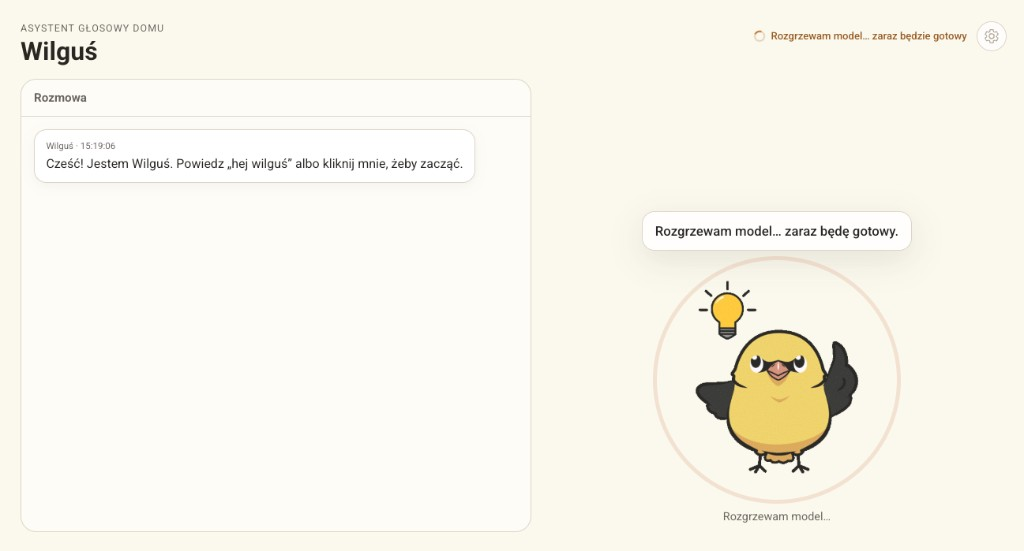
\includegraphics[width=\textwidth]{src/img/app_warmup.png}
    \caption{Faza rozgrzewania modelu Ucznia. Interfejs informuje
             o~ładowaniu wag i~KV-cache, zanim możliwe będzie zapytanie
             bez kosztu \emph{cold cache}.}
    \label{fig:app_warmup}
\end{figure}

Po zakończeniu procesu rozgrzewania modelu Ucznia użytkownikowi prezentowany jest delikatnie inny widok-  ekran startowy
(rysunek~\ref{fig:app_start}): powitanie, subtelne instrukcje jak rozpocząć rozmowę (raza startowa lub kliknięcie Wilgusia). Dodatkow aby zachęcić do interakcji postać Wilgusi pulsuje pokazując swoją gotowość do interakcji. Widok startowy nadal trzyma omówiony powyżej dwukolumnowy układ.

\begin{figure}[H]
    \centering
    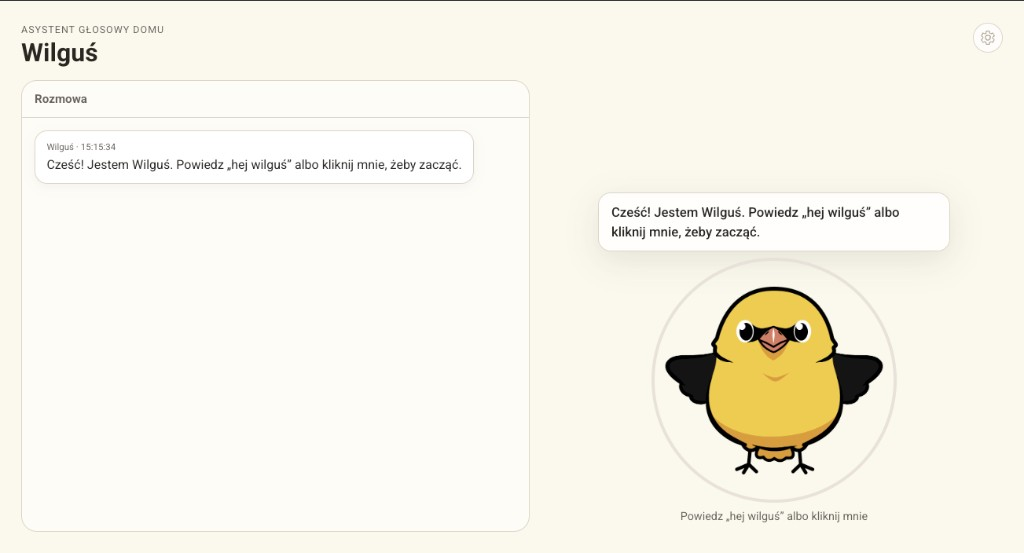
\includegraphics[width=\textwidth]{src/img/app_start.png}
    \caption{Ekran startowy po rozgrzaniu modelu: karta historii rozmowy
             oraz interaktywna postać Wilguś.}
    \label{fig:app_start}
\end{figure}

Wilguś widoczny w prawej kolumnie prezentowanych widoków nie jest statyczną ilustracją. Tablica \texttt{WILGUS\_BY\_STATUS}
przypisuje fazom czy statusom aplikacji osobną grafikę dynamiczną i~podpis, dzięki czemu postać
sygnalizuje, co system właśnie robi. Grafiki zapisane w formacie GIF wprowadzają element ruchu, który podnosi zaangażowanie użytkownika. Klatki faz używanych w~prototypie
zestawiono na rysunku~\ref{fig:wilgus_fazy}. Postać Wilgusia została zaprojektowana przez Julię Nazarską, studentkę wydziały Architektury Politechniki Warszawskiej.

\begin{figure}[H]
    \centering
    \begin{minipage}[t]{0.18\textwidth}
        \centering
        
\includegraphics[width=\linewidth]{src/img/wilgus/wilgus_neutral.png}\\[0.4em]
        {\small gotowy / \textit{hej wilguś}}
    \end{minipage}
    \hfill
    \begin{minipage}[t]{0.18\textwidth}
        \centering
        
\includegraphics[width=\linewidth]{src/img/wilgus/wilgus_macha.png}\\[0.4em]
        {\small słucham dalej}
    \end{minipage}
    \hfill
    \begin{minipage}[t]{0.18\textwidth}
        \centering
        
\includegraphics[width=\linewidth]{src/img/wilgus/wilgus_zdziwiony.png}\\[0.4em]
        {\small nagrywam}
    \end{minipage}
    \hfill
    \begin{minipage}[t]{0.18\textwidth}
        \centering
        
\includegraphics[width=\linewidth]{src/img/wilgus/wilgus_pomysl.png}\\[0.4em]
        {\small myślę}
    \end{minipage}
    \hfill
    \begin{minipage}[t]{0.18\textwidth}
        \centering
        
\includegraphics[width=\linewidth]{src/img/wilgus/wilgus_gada.png}\\[0.4em]
        {\small mówię}
    \end{minipage}
    \caption{Stany Wilgusia w aplikacji użytkownika.}
    \label{fig:wilgus_fazy}
\end{figure}

Podczas konwersacji lewa kolumna wypełnia się wiadomościami użytkownika i odpowiedziami asystenta. Całość ma przypominać dobrze znany interfejs chatu, przez co korzystanie z aplikacji jest intuicyjne. Na rysunku~\ref{fig:app_rozmowa} przedstawiono przykładowy widok w trakcie prowadzenia rozmowy.

\begin{figure}[H]
    \centering
    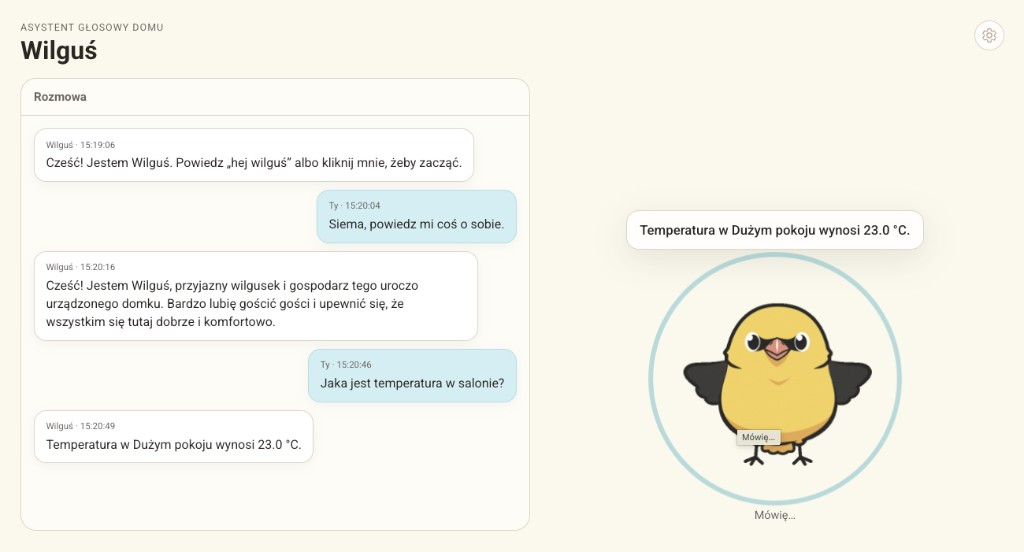
\includegraphics[width=\textwidth]{src/img/app_rozmowa.png}
    \caption{Widok aplikacji w trakcie prowadzenia rozmowy.}
    \label{fig:app_rozmowa}
\end{figure}

\subsubsection{Transkrypcja mowy (STT)}

Za transkrypcję mowy, czyli element procesu nazwany STT na schemacie architektonicznym (rysunek~\ref{fig:architektura}) odpowiada blok roboczo nazwany Whisper Backend. Jest to usługa stworzono w oparciu o bliblitekę języka Python FastAPI oraz otwartoźródłowego modelu Whisper. Sercem moduły jest transkrypcja, którą realizuje biblioteka \texttt{faster-whisper} \cite{Radford2023}. W prezentowanym rozwiązaniu zdecydowano się implementować wa
wariant \texttt{small}, oczywiście w konfiguracji wskazano język polski (\texttt{pl}). Filtr VAD po stronie Whisper jest wyłączony
(\texttt{WHISPER\_VAD\_FILTER=false}), ponieważ w systemie istnieje własny detektor aktywności, widoczny na schemacie architektornicznym pod nazwa \texttt{VAD}.

Nagranie zebrane przez aplikację użytkownika zostaje wysłane do Whisper Backendu poprzez żądanie HTTP \texttt{POST /api/transcribe},
pole \texttt{file}) zawiera plik nagrania (mechanizm znany z formularzy aplikacji webowych \texttt{multipart/form-data})). Odpowiedź zwracana jest w formacie JSON, jej przykład przedstawiono poniżej:

\begin{verbatim}
{"text": "jaka jest temperatura w salonie",
 "language": "pl",
 "duration_seconds": 2.4}
\end{verbatim}

Moduł STT został zabezpieczony przez błedami. Serwis odrzuca nagrania większe niż 25~MB oraz niemal puste pliki
(poniżej ok.\ 1{,}5~kB), brak reakcji na szum. 

\subsubsection{Context Engine}
\label{subsec:kontekst}

Context Engine jest zestawem skryptów Python opakowanych w~FastAPI
na porcie \texttt{8001}. Ponieważ instalacja IoT w~Wildze nie dostarczała
strumienia na żywo w~trakcie prac, serwis czyta historyczny CSV
z~\texttt{db\_sampler} (okres 31.10.2025--27.01.2026, 147~kolumn
wraz z~polem czasu).
Każdy cykl odświeżania przesuwa kursor o~jeden wiersz (w~danych jest to
krok ok.~5~minut); po ostatnim wierszu symulacja wraca na początek.
Do promptu nie idzie pełna szerokość tabeli --- parser zostawia metryki
komfortu i~stanu technicznego (temperatura, wilgotność, obecność,
kontaktrony, oświetlenie, moc, energia, VOC) i~pomija m.in.\ baterie
oraz jakość łącza, żeby nie rozdymać okna kontekstu Ucznia.

Fakty dla Ucznia składa warstwa deterministyczna: z~wiersza CSV powstaje
punktowy \emph{snapshot} z~etykietami pomieszczeń (łazienka, duży pokój,
mały pokój, korytarz). Model językowy nie liczy progów ani stanów
boolowskich. Nauczyciel dostaje ten sam snapshot wyłącznie po to,
by zgłosić anomalie. Jeśli wywołanie się nie uda, fakty i~tak zostają
opublikowane --- serwis nie blokuje asystenta na awarii większego modelu.

Kontekst ma dwa bufory. \emph{Published} jest przypięty do bieżącej
rozmowy; \emph{staging} odświeża się w~tle. Nowa sesja
(\texttt{POST /api/session/new} po stronie Whisper Backendu) woła
\texttt{POST /api/context/advance} i~przestawia publikowany snapshot
na nowszy, bez zmiany stałego prefiksu reguł. Dzięki temu KV-cache
prefiksu na Pi pozostaje ważny między turami.

Whisper Backend pobiera bieżący kontekst przez
\texttt{GET /api/context}. Przykładowa odpowiedź:

\begin{verbatim}
{
  "status": "ready",
  "source_timestamp": "2025-11-01T12:00:00Z",
  "static_prefix": "Jesteś Wilguś — ...",
  "dynamic_context": "Stan mieszkania na ... UTC: ...",
  "system_prompt": "Jesteś Wilguś — ...\n\nStan mieszkania...",
  "insight": "Okno w korytarzu otwarte."
}
\end{verbatim}

Pole \texttt{static\_prefix} (persona i~reguły) jest niezmienne między
zapytaniami. Pole \texttt{dynamic\_context} to fakty plus opcjonalna
sekcja Findings. Pole \texttt{system\_prompt} jest złożeniem obu części,
zostawionym dla zgodności wstecznej. Przy \texttt{status: pending}
(pierwszy cykl po starcie) backend nie czeka w~nieskończoność:
używa zapasowego prefiksu wbudowanego w~Whisper Backend i~może
odpowiadać bez faktów, zamiast blokować cały interfejs.

\subsubsection{LLM Nauczyciel}

Nauczyciel działa lokalnie na Macu przez Ollamę
(adres w~\texttt{TEACHER\_OLLAMA\_URL}, model \texttt{qwen2.5}),
z~\texttt{keep\_alive} równym 30~min i~bez strumieniowania. Zadanie jest wąskie:
nie streszczać całego domu, tylko wskazać odchylenia (skrajne temperatury,
otwarte okna, nietypowa obecność, wysokie VOC, sprzeczne odczyty).
Gdy nic nie zasługuje na uwagę, model ma zwrócić dokładnie jedną linię
\texttt{BRAK\_ANOMALII}; serwis traktuje to jako brak findings
i~nie dokleja sekcji do promptu Ucznia.

Żądanie do Ollamy ma postać:

\begin{verbatim}
{
  "model": "qwen2.5",
  "messages": [
    {"role": "system", "content": "Jesteś analitykiem IoT smart-home..."},
    {"role": "user",   "content": "Snapshot czujników z ..."}
  ],
  "stream": false,
  "keep_alive": "30m"
}
\end{verbatim}

\subsubsection{SLM Uczeń}

Uczeń to \texttt{gemma3:4b} na Raspberry~Pi (Ollama API w~sieci lokalnej),
w~konfiguracji z~tabeli~\ref{tab:rekomendacja_produkcyjna}. Zapytanie
z~frontendu to \texttt{POST /api/chat}:

\begin{verbatim}
{
  "message": "Jaka jest temperatura w salonie?",
  "history": [
    {"role": "user", "content": "Siema, powiedz mi coś o sobie"},
    {"role": "assistant", "content": "Jestem Wilguś, gospodarz domku..."}
  ]
}
\end{verbatim}

Backend dokłada co najwyżej ostatnie sześć tur historii
(\texttt{CHAT\_HISTORY\_MAX\_MESSAGES}). Payload do Ollamy rozdziela
role tak, by prefiks systemowy był bitowo stały: najpierw
\texttt{role: system} ze \texttt{static\_prefix}, potem --- jeśli są ---
fakty domu jako osobna wiadomość użytkownika, następnie historia
i~bieżące pytanie. Włączenie \texttt{stream: true} oraz
\texttt{keep\_alive} z~konfiguracji pozwala strumieniować tokeny
i~utrzymać ciepły cache. Odpowiedź do przeglądarki idzie jako NDJSON:

\begin{verbatim}
{"type":"chunk","content":"Temperatura w Dużym pokoju"}
{"type":"chunk","content":" wynosi 23,0 °C."}
{"type":"done"}
\end{verbatim}

Zdarzenie \texttt{error} pojawia się przy przekroczeniu limitu czasu
Ollamy (120~s, HTTP~504 na etapie połączenia) albo przy błędzie sieci.
Gdy Context Service nie odpowiada, Uczeń dostaje wyłącznie zapasowy
prefiks persony i~odmawia cytowania liczb spoza faktów --- zgodnie
z~regułami promptu.

\subsubsection{Synteza mowy (TTS)}

Frontend tnie napływające zdania i~kolejkuje
\texttt{POST /api/tts} z~ciałem \texttt{\{"text": "..."\}}.
Odpowiedź to \texttt{audio/mpeg}. Syntezę realizuje \texttt{edge-tts}
\cite{EdgeTTS} głosem \texttt{pl-PL-ZofiaNeural}; wymaga to sieci
wychodzącej do usług Microsoft. Limit długości wynosi 1000~znaków.
Takie podejście daje akceptowalną jakość polszczyzny bez trenowania
własnego TTS, przy czym sam Uczeń nadal liczy się wyłącznie lokalnie.

\subsubsection{Konfiguracja}

Adresy, nazwy modeli i~interwały siedzą w~plikach \texttt{.env},
bez zmian w~kodzie:

\begin{itemize}
    \item \texttt{context\_service/.env}: \texttt{TEACHER\_OLLAMA\_URL},
          \texttt{TEACHER\_OLLAMA\_MODEL}, \texttt{CONTEXT\_REFRESH\_INTERVAL},
          \texttt{SENSOR\_DATA\_PATH};
    \item \texttt{whisper-proj/backend/.env}: \texttt{OLLAMA\_URL},
          \texttt{OLLAMA\_MODEL}, \texttt{CONTEXT\_SERVICE\_URL},
          \texttt{WHISPER\_MODEL\_SIZE}, \texttt{OLLAMA\_KEEP\_ALIVE},
          \texttt{TTS\_VOICE}.
\end{itemize}

\subsection{Testy rozwiązania}
\label{subsec:testy_prototypu}

Pełny stos uruchamia skrypt \texttt{start.sh}: lokalna Ollama Nauczyciela,
Context Service, Whisper Backend i~serwer deweloperski frontendu.
Przed startem skrypt sprawdza \texttt{/api/tags} obu instancji Ollamy,
obecność modeli oraz środowiska Python; Nauczyciela rozgrzewa od razu,
Ucznia --- pętla keep-warm w~backendzie, ta sama która steruje
rysunkiem~\ref{fig:app_warmup}.

Odporność na typowe awarie wbudowano w~ścieżkę żądania, a~nie w~osobny
moduł. Brak pierwszego snapshotu zgłasza \texttt{status: pending};
niedostępny Context Service spada na zapasowy prefiks; pad Nauczyciela
zostawia fakty bez Findings; rozgrzewający się Uczeń wraca 503;
przekroczenie czasu Ollamy --- 504. Interwał keep-warm (10~min) jest
krótszy niż \texttt{keep\_alive} (30~min), żeby model nie wypadł
z~pamięci między turami.

Poprawność łańcucha sprawdzano ręcznie: uruchomienie aplikacji
i~rozmowy głosowe oraz tekstowe, w~scenariuszach zbliżonych do złotego
zbioru z~części badawczej --- pytanie o~stan (temperatura, oświetlenie),
brak danych (oczekiwana odmowa zamiast halucynacji) oraz nieaktualny
znacznik czasu. W~pracy tekstowej nie zamieszcza się nagrań sesji;
zrzuty na rysunkach~\ref{fig:app_start}--\ref{fig:app_rozmowa} dokumentują
układ i~przykładową turę, nie pełną ewaluację jakości.

Czasy odpowiedzi w~prototypie mieszczą się w~rzędzie wielkości
zmierzonych dla konfiguracji produkcyjnej: przy \emph{warm cache}
mediana E2E modelu LN wynosi ok.~9~s
(tabela~\ref{tab:rekomendacja_produkcyjna}). Bez rozgrzania i~stałego
prefiksu ten sam węzeł wraca do opóźnień cold-cache omówionych
w~sekcji~\ref{subsec:kwantyzacja}.
